% !TeX program = xelatex
% 三組新增圖片，依註解位置分別貼入學姐的章節檔。
% 將 figsrc/ch01/ 內對應圖檔上傳至相同路徑。
% 將「thesis_references.bib」中尚未存在的項目加入 thesis.bib。
% 不需新增 chapter、section，亦不需額外加入 subcaption 等套件。

% 建議位置：1.1.1，介紹移動機械臂組成與應用領域的段落後。
移動機械臂可依應用需求採用不同的機構配置，如\cref{fig:mobile_manipulator_applications}所示。KUKA KMR iisy 結合移動平台與機械手臂，支援生產及物流場域的跨站作業；Hello Robot Stretch 則以室內環境中的移動與物件互動為主要設計方向\cite{kukakmriisy,hellorobotstretch4}。
\begin{figure}[htbp]
    \centering
    \begin{minipage}[b]{0.49\textwidth}
        \centering
        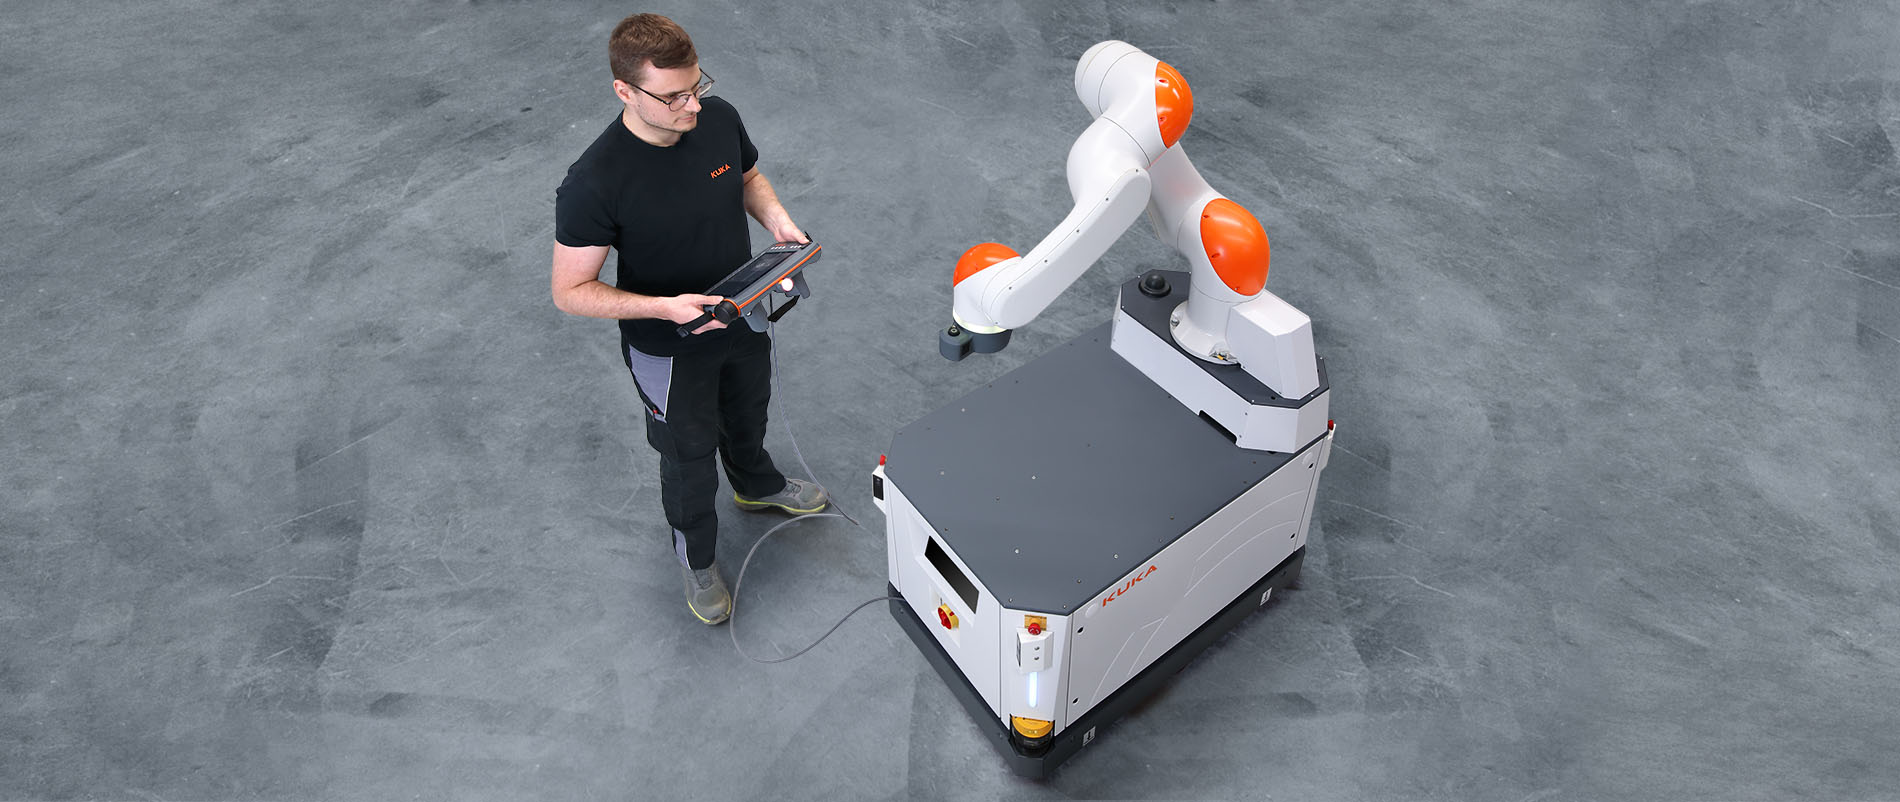
\includegraphics[width=\linewidth,height=3.2cm,keepaspectratio]{figsrc/ch01/kuka_kmr_iisy_application.jpg}
        \par\smallskip
        {\small (a) KUKA KMR iisy}
    \end{minipage}\hfill
    \begin{minipage}[b]{0.49\textwidth}
        \centering
        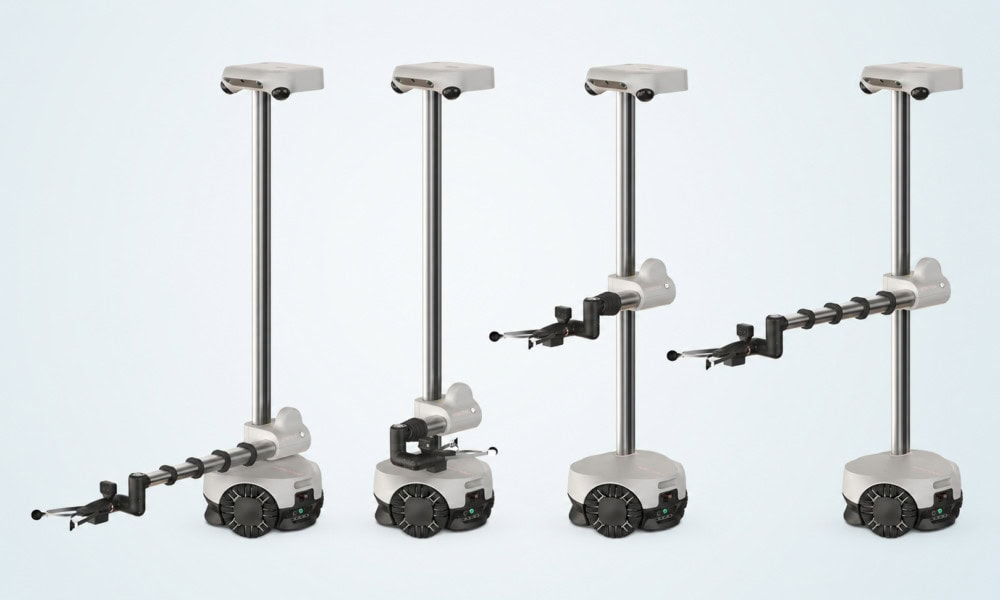
\includegraphics[width=\linewidth,height=3.2cm,keepaspectratio]{figsrc/ch01/stretch4_platform_views.jpg}
        \par\smallskip
        {\small (b) Hello Robot Stretch 4}
    \end{minipage}
    \caption{工業與室內應用導向之移動機械臂平台實例\cite{kukakmriisy,hellorobotstretch4}}
    \label{fig:mobile_manipulator_applications}
\end{figure}

% 建議位置：1.1.2，說明門扇、櫃門及抽屜等機構操作需求的段落後。
室內操作的對象包含受鉸鏈或滑軌限制的可動機構，其允許的運動方向與自由空間中的物件搬運不同。Mittal 等人\cite{mittal2022articulated}以不同形式的移動機械臂處理關節式物件互動，相關研究情境如\cref{fig:articulated_object_examples}所示，呈現感知、移動與操作協調的需求。
\begin{figure}[htbp]
    \centering
    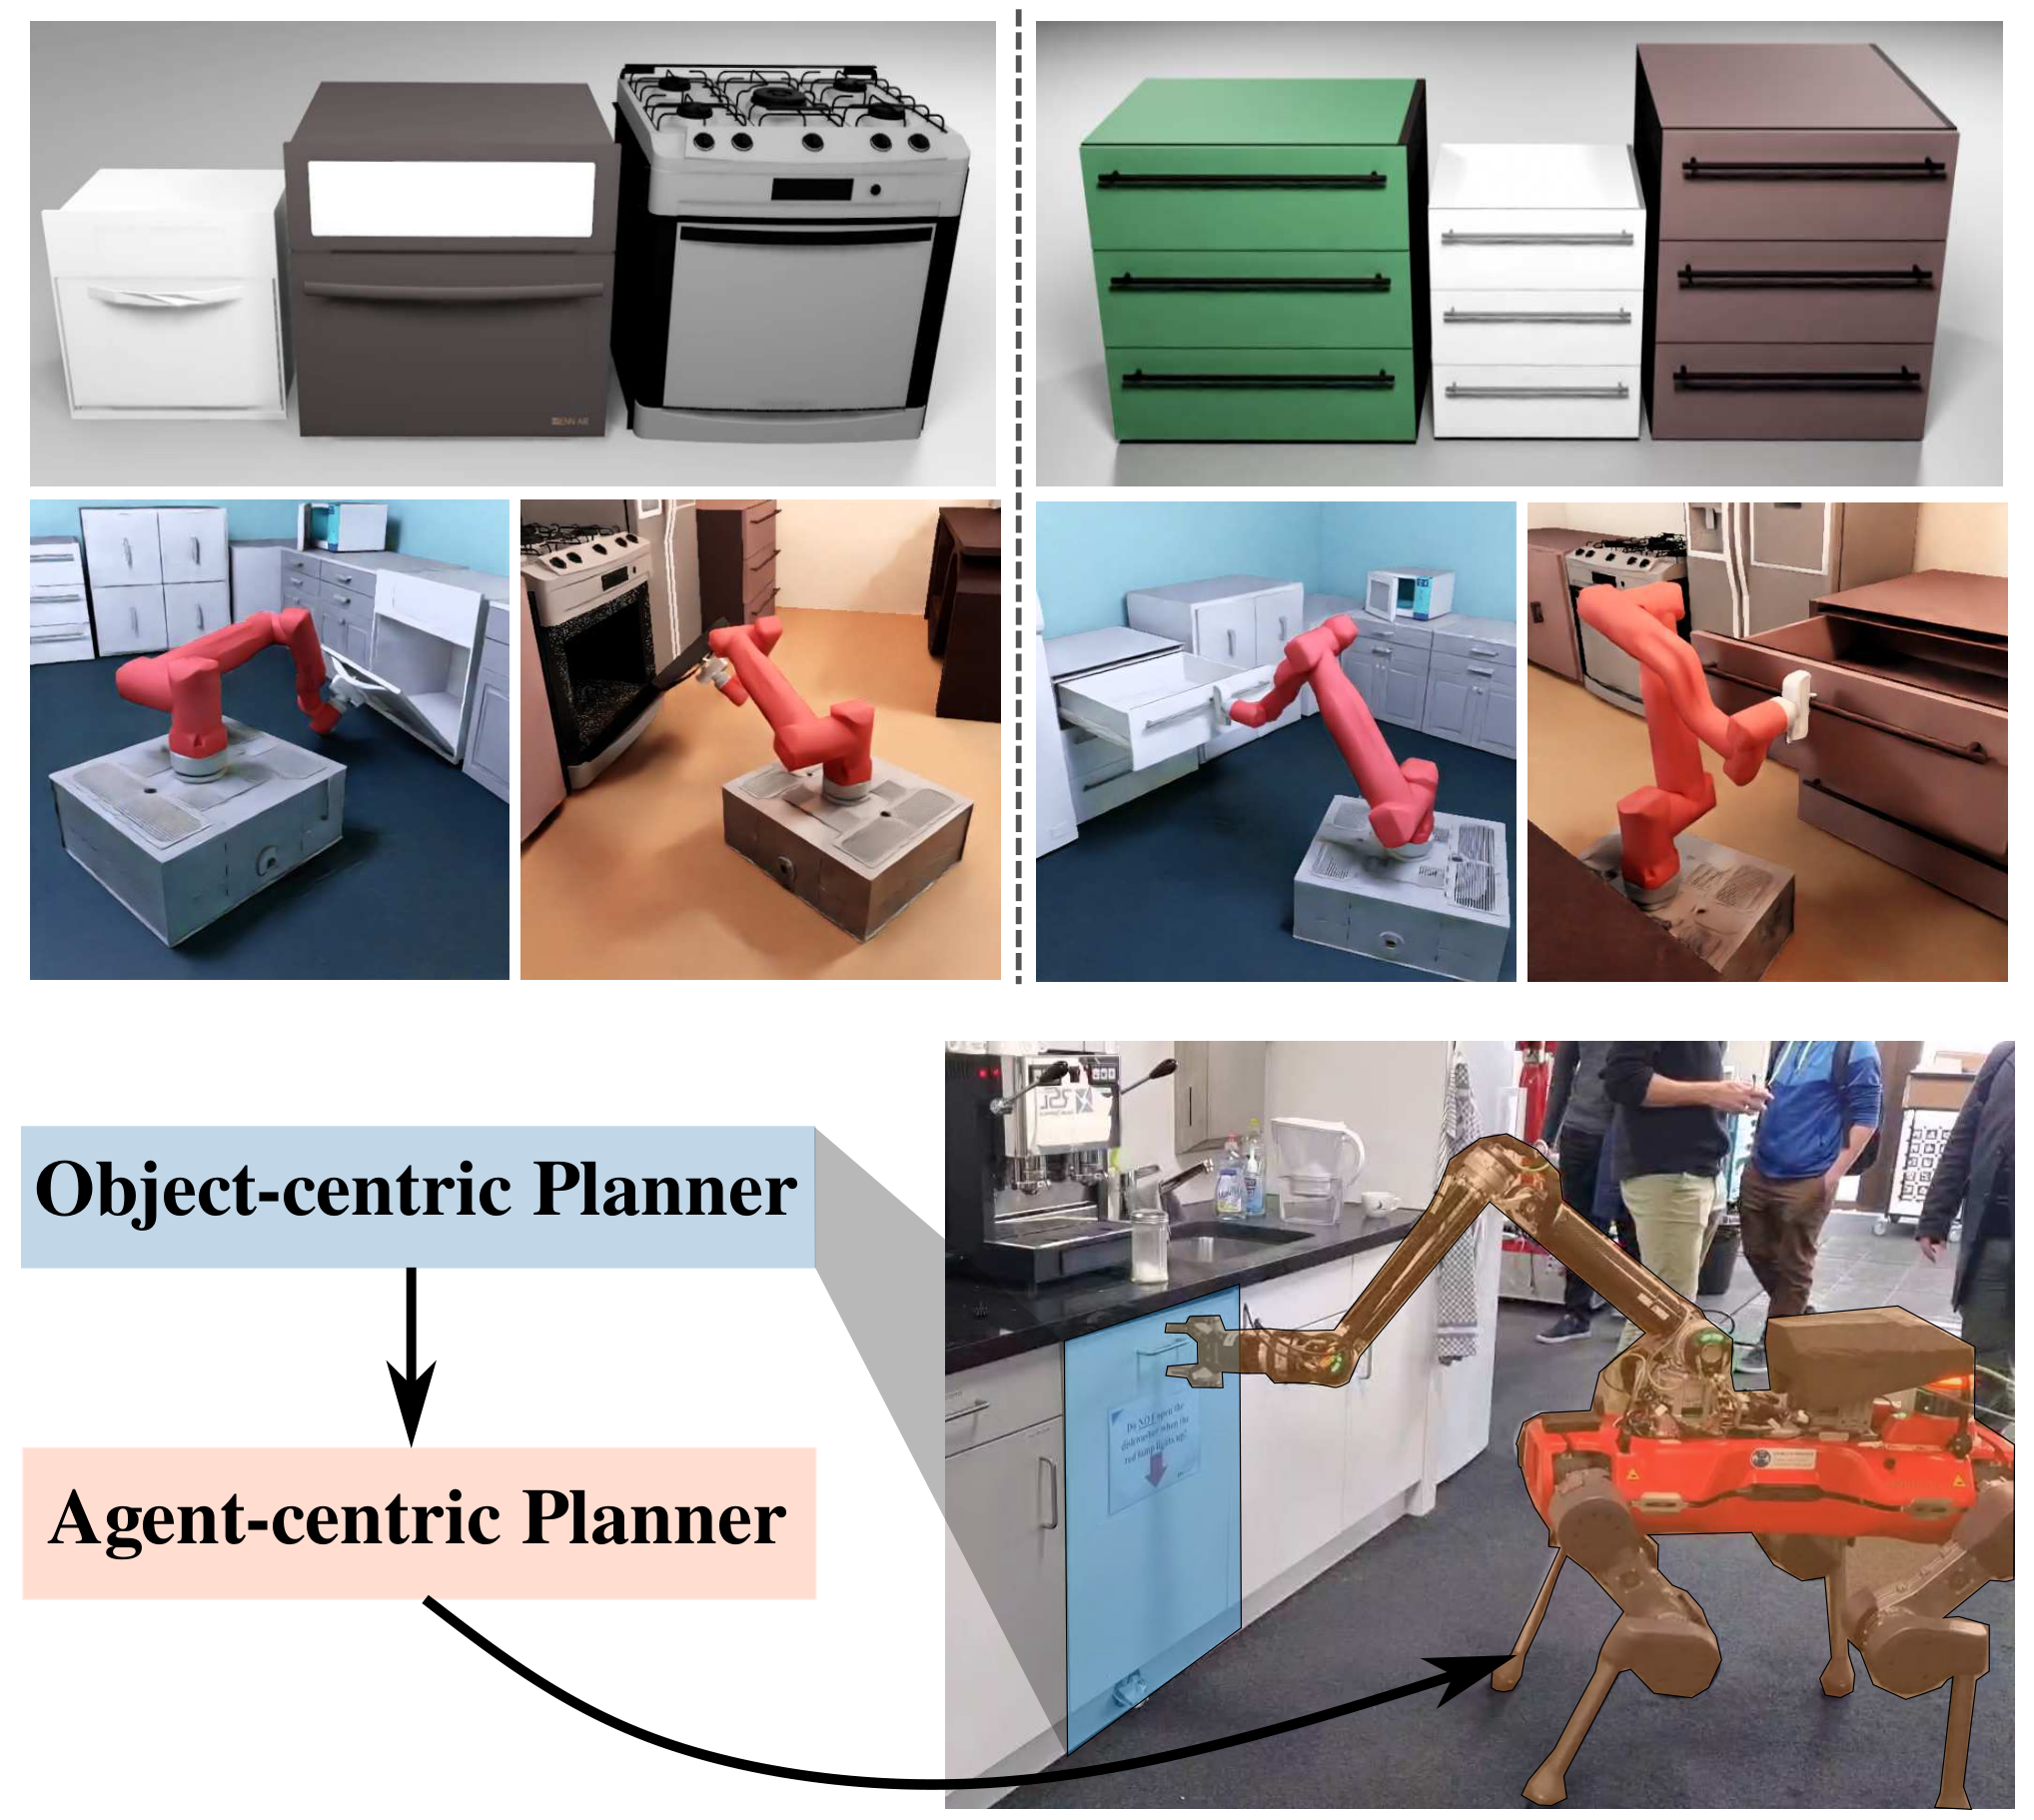
\includegraphics[width=0.80\textwidth]{figsrc/ch01/mittal2022_articulated_fig1.png}
    \caption{關節式物件操作之研究情境與系統示意，含模擬與實機場景\cite{mittal2022articulated}}
    \label{fig:articulated_object_examples}
\end{figure}

% 建議位置：1.3.2「全身模型預測控制與移動中操作」，介紹 MotM 的段落後。
移動中操作使底盤行進與手臂動作在時間上重疊，需協調機器人與操作目標之相對運動。Burgess-Limerick 等人\cite{burgess2023motm}提出反應式移動操作架構，其作者專案提供的連續動作示意如\cref{fig:motm_research_example}所示\cite{burgessmotmproject}。
\begin{figure}[htbp]
    \centering
    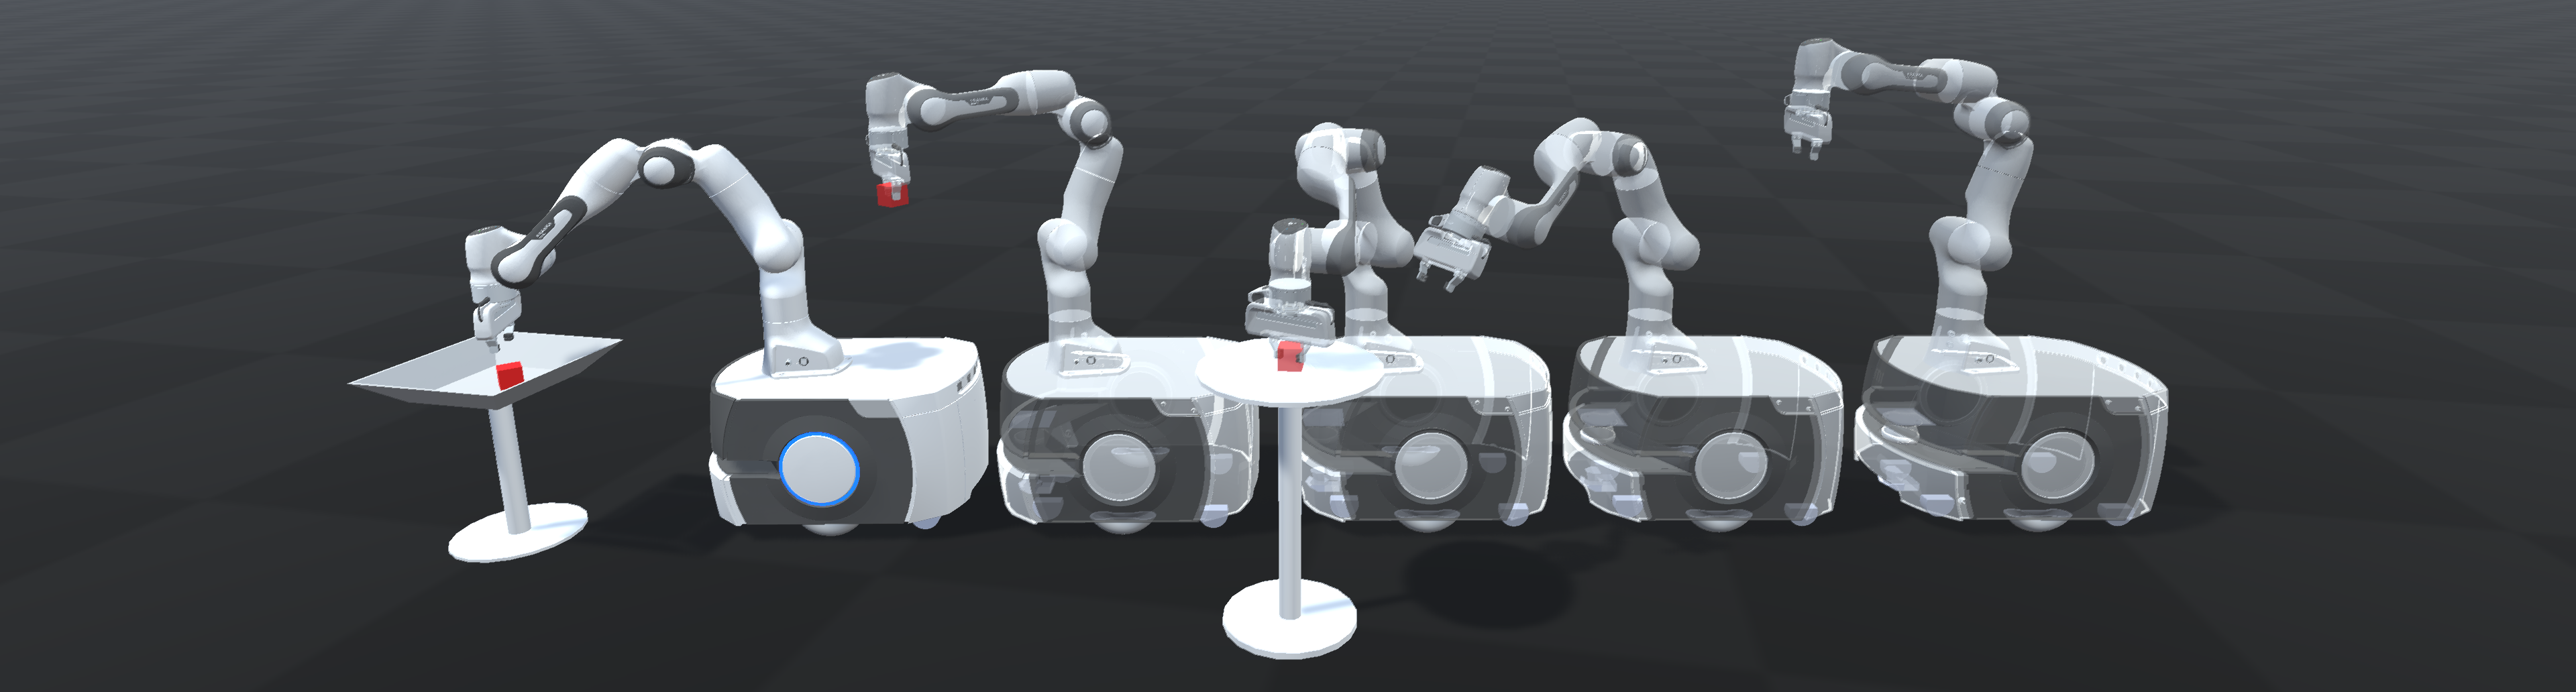
\includegraphics[width=1.0\textwidth]{figsrc/ch01/burgess2023_motm_banner.png}
    \caption{移動中抓取與放置之連續動作示意，取自作者專案之模擬圖\cite{burgess2023motm,burgessmotmproject}}
    \label{fig:motm_research_example}
\end{figure}
